% This LaTeX document needs to be compiled with XeLaTeX.
\documentclass[10pt]{article}
\usepackage[utf8]{inputenc}
\usepackage{amsmath}
\usepackage{amsfonts}
\usepackage{amssymb}
\usepackage[version=4]{mhchem}
\usepackage{stmaryrd}
\usepackage{bbold}
\usepackage{graphicx}
\usepackage[export]{adjustbox}
\graphicspath{ {./images/} }
\usepackage[fallback]{xeCJK}
\usepackage{polyglossia}
\usepackage{fontspec}
\IfFontExistsTF{Noto Serif CJK TC}
{\setCJKmainfont{Noto Serif CJK TC}}
{\IfFontExistsTF{STSong}
  {\setCJKmainfont{STSong}}
  {\IfFontExistsTF{Droid Sans Fallback}
    {\setCJKmainfont{Droid Sans Fallback}}
    {\setCJKmainfont{SimSun}}
}}

\setmainlanguage{spanish}
\IfFontExistsTF{CMU Serif}
{\setmainfont{CMU Serif}}
{\IfFontExistsTF{DejaVu Sans}
  {\setmainfont{DejaVu Sans}}
  {\setmainfont{Georgia}}
}

\begin{document}
\section*{Existencia}
\section*{1. El principio de los casilleros.}
Si queremos colocar 13 bolillas en 12 cajas, es evidente que en alguna caja deberemos colocar al menos dos bolillas. Lo mismo ocurre si en lugar de 13 bolillas tuviésemos 17. Y también si tuviésemos 25. Más aún, si tuviésemos 25 bolillas entonces podemos asegurar que en alguna caja deberemos colocar al menos 3 . Este es un caso particular del siguiente teorema, conocido como el principio de los casilleros.

Teorema: (Principio de los casilleros) Sean $A$ y $B$ dos conjuntos finitos no vacíos y sea $\mathcal{R}$ una relación de $A$ en $B$. Entonces se verifican:\\
i) $\exists a \in A$ tal que $|\mathcal{R}(a)| \geq \frac{|\mathcal{R}|}{|A|}$\\
ii) $\exists a \in A$ tal que $|\mathcal{R}(a)| \leq \frac{|\mathcal{R}|}{|A|}$\\
iii) $\exists b \in B$ tal que $\left|\mathcal{R}^{-1}(b)\right| \geq \frac{|\mathcal{R}|}{|B|}$\\
iv) $\exists b \in B$ tal que $\left|\mathcal{R}^{-1}(b)\right| \leq \frac{|\mathcal{R}|}{|B|}$\\
donde $\mathcal{R}(a)=\{b \in B /(a, b) \in \mathcal{R}\}$ y $\mathcal{R}^{-1}$ denota la relación inversa de $\mathcal{R}$.\\
Demostración: Como $\mathcal{R}=\bigcup_{a \in A}(\{a\} \times \mathcal{R}(a))$ y esta unión es disjunta entonces se tiene que $|\mathcal{R}|=\sum_{a \in A}|\mathcal{R}(a)|$.\\
i) Si fuese $|\mathcal{R}(a)|<\frac{|\mathcal{R}|}{|A|}$ para todo $a \in A$ entonces se tendría que

$$
|\mathcal{R}|=\sum_{a \in A}|\mathcal{R}(a)|<\sum_{a \in A} \frac{|\mathcal{R}|}{|A|}=|A| \cdot \frac{|\mathcal{R}|}{|A|}=|\mathcal{R}|
$$

lo cual es un absurdo.\\
ii) Idem i) cambiando < por >\\
iii) Aplicar i) a la relación $\mathcal{R}^{-1}$ y observar que $\left|\mathcal{R}^{-1}\right|=|\mathcal{R}|$\\
iv) Aplicar ii) a la relación $\mathcal{R}^{-1}$ 口

Ejemplo: Sea $S$ un conjunto con 100 elementos y sean $A_{1}, \ldots, A_{50}$ subconjuntos distintos de $S$ con 40 elementos cada uno. Entonces existe $x \in S$ tal que $x$ pertenece a por lo menos 20 de los conjuntos $A_{i}$.

En efecto, si definimos una relación $\mathcal{R}$ de $\left\{A_{1}, \ldots, A_{50}\right\}$ en $S$ en la forma

$$
\left(A_{i}, s\right) \in \mathcal{R} \text { si y sólo si } s \in A_{i}
$$

resulta que, por el principio de los casilleros, existe $x \in S$ tal que

$$
\left|\mathcal{R}^{-1}(x)\right| \geq \frac{|\mathcal{R}|}{|S|}=\frac{50.40}{100}=20
$$

Luego, existe $x \in S$ tal que

$$
\left|\left\{A_{i} / x \in A_{i}\right\}\right|=\left|\left\{A_{i} /\left(A_{i}, x\right) \in \mathcal{R}\right\}\right|=\left|\left\{A_{i} /\left(x, A_{i}\right) \in \mathcal{R}^{-1}\right\}\right|=\left|\mathcal{R}^{-1}(x)\right| \geq 20
$$

Veamos ahora qué sucede con el principio de los casilleros en el caso particular en que la relación es una función de $A$ en $B$. Si $f: A \longrightarrow B$ es una función de $A$ en $B$ entonces $|f|=\sum_{a \in A}|f(a)|=|A|$ pues $|f(a)|=1$ para todo $a \in A$. Luego, i) dice que existe $a \in A$ tal que $1 \geq \frac{|A|}{|A|}$ y ii) dice que existe $a \in A$ tal que $1 \leq \frac{|A|}{|A|}$. Esto significa que i) y ii) no aportan ninguna información. Pero iii) y iv) se traducen en:\\
iii) $\exists b \in B$ tal que $\left|f^{-1}(b)\right| \geq \frac{|A|}{|B|}$\\
iv) $\exists b \in B$ tal que $\left|f^{-1}(b)\right| \leq \frac{|A|}{|B|}$\\
donde $f^{-1}(b)=\{a \in A / f(a)=b\}$\\
Ejemplo: Sean $A, B$ y $C$ tres conjuntos disjuntos. Entonces cualquier subconjunto de 5 elementos de $A \cup B \cup C$ contiene tres elementos del mismo conjunto ( $A$ o $B$ o $C$ ) o un elemento de cada uno.\\
En efecto, supongamos que $U=\left\{x_{1}, x_{2}, x_{3}, x_{4}, x_{5}\right\}$ es un subconjunto de 5 elementos de $A \cup B \cup C$. Si $U$ no contiene ningún elemento de $A$ entonces podemos definir una función $f: U \longrightarrow\{B, C\}$ en la forma:

$$
f\left(x_{i}\right)= \begin{cases}B & \text { si } x_{i} \in B \\ C & \text { si } x_{i} \in C\end{cases}
$$

Luego, $\left|f^{-1}(B)\right| \geq \frac{5}{2}>2$ o $\left|f^{-1}(C)\right| \geq \frac{5}{2}>2$, de donde $\left|f^{-1}(B)\right| \geq 3$ o $\left|f^{-1}(C)\right| \geq 3$. Luego hay al menos tres elementos de $U$ que pertenecen al mismo conjunto. Lo mismo ocurre si $U$ no contiene ningún elemento de $B$ o ningún elemento de $C$.

Observación: Si $f: A \longrightarrow B$ es una función y $|A|>|B|$ entonces $\exists b \in B$ tal que $\left|f^{-1}(b)\right| \geq 2$, es decir, $\exists a_{1}, a_{2} \in A, a_{1} \neq a_{2}$, tales que $f\left(a_{1}\right)=f\left(a_{2}\right)$. El caso particular\\
en que $|A|=|B|+1$ puede interpretarse de la siguiente manera: "si $k+1$ objetos son colocados en $k$ casilleros entonces algún casillero debe contener al menos dos objetos".

Ejemplo: Llamaremos lattice points a los puntos del plano que tienen ambas coordenadas enteras. Veremos que dados 5 lattice points $p_{1}, \ldots, p_{5}$ en el plano, hay (al menos) dos de ellos tales que el punto medio del segmento que los une es también un lattice point. Para ello, definimos la función $f:\left\{p_{1}, \ldots, p_{5}\right\} \longrightarrow\{(0,0),(0,1),(1,0),(1,1)\}$ en la forma:

$$
\text { si } p_{i}=\left(a_{i}, b_{i}\right) \text { entonces } f\left(p_{i}\right)=\left(r_{2}\left(a_{i}\right), r_{2}\left(b_{i}\right)\right)
$$

donde $r_{2}(a)$ denota el resto de la división de $a$ por 2 . Luego, por la observación, $\exists i \neq j$ tales que $f\left(p_{i}\right)=f\left(p_{j}\right)$. Por lo tanto $r_{2}\left(a_{i}\right)=r_{2}\left(a_{j}\right)$ y $r_{2}\left(b_{i}\right)=r_{2}\left(b_{j}\right)$, de donde $a_{i}+a_{j}$ y $b_{i}+b_{j}$ son pares.\\
Luego, el punto medio del segmento que une $p_{i}$ con $p_{j}$, que es $\left(\frac{a_{i}+a_{j}}{2}, \frac{b_{i}+b_{j}}{2}\right)$, tiene ambas coordenadas enteras.

Notar que para 4 puntos el resultado anterior es falso: si consideramos los lattice points $p_{1}=(0,0), p_{2}=(0,1), p_{3}=(1,0)$ y $p_{4}=(1,1)$ entonces el punto medio de segmento que une dos cualesquiera de estos puntos nunca es un lattice point.

Teorema: Dados $\alpha \in \mathbb{R}$ y $n \in \mathbb{N}$ existen $p, q \in \mathbb{Z}$ tales que $1 \leq q \leq n$ y $\left|\alpha-\frac{p}{q}\right|<\frac{1}{n \cdot q}$\\
Demostración: Sea

$$
f:\{1,2, \ldots, n, n+1\} \longrightarrow\left\{\left[0, \frac{1}{n}\right),\left[\frac{1}{n}, \frac{2}{n}\right), \ldots,\left[\frac{n-1}{n}, 1\right)\right\}
$$

la función definida por

$$
f(j)=\left[\frac{k}{n}, \frac{k+1}{n}\right) \text { si y sólo si } j \alpha-[j \cdot \alpha] \in\left[\frac{k}{n}, \frac{k+1}{n}\right) \quad(0 \leq k \leq n-1)
$$

donde $[j . \alpha]$ denota la parte entera de $j . \alpha$\\
Notar que $f$ está bien definida pues $j . \alpha-[j . \alpha]$ pertenece al intervalo $[0,1)$ que es la unión disjunta de los intervalos $\left[\frac{k}{n}, \frac{k+1}{n}\right) \quad(0 \leq k \leq n-1)$.\\
Por la observación, $\exists j>i,(1 \leq j, i \leq n+1)$ tales que $f(j)=f(i)$. Sea $k, 0 \leq k \leq n-1$, tal que $f(j)=\left[\frac{k}{n}, \frac{k+1}{n}\right)=f(i)$. Entonces $j . \alpha-[j . \alpha] \in\left[\frac{k}{n}, \frac{k+1}{n}\right)$ e $i . \alpha-[i . \alpha] \in\left[\frac{k}{n}, \frac{k+1}{n}\right)$ de donde $|(j . \alpha-[j . \alpha])-(i . \alpha-[i . \alpha])|<\frac{1}{n}$\\
Tomando $p=[j . \alpha]-[i . \alpha]$ y $q=j-i$ resulta que $p, q \in \mathbb{Z}, 1 \leq q \leq n$ y

$$
q \cdot\left|\alpha-\frac{p}{q}\right|=|q \cdot \alpha-p|=|j \cdot \alpha-i \cdot \alpha-[j \cdot \alpha]+[i \cdot \alpha]|=|(j \cdot \alpha-[j \cdot \alpha])-(i \cdot \alpha-[i \cdot \alpha])|<\frac{1}{n}
$$

es decir, $\left|\alpha-\frac{p}{q}\right|<\frac{1}{n \cdot q}$ ㅁ\\
Este teorema garantiza la existencia de un número racional $\frac{p}{q}$ que aproxima "bien" a un dado número irracional $\alpha$.

Definición: Un grafo es un par ( $V, E$ ) donde $V$ es un conjunto finito y $E$ es un conjunto de pares de elementos distintos de $V$. Llamaremos vértices o nodos a los elementos de $V$ y ramas o arcos a los elementos de $E$. Cuando nos importe el orden en las ramas (es decir, cuando las ramas sean pares ordenados de elementos distintos de $V$ ) diremos que el grafo es dirigido. En caso contrario, (es decir, cuando las ramas sean pares no ordenados) diremos que el grafo es no dirigido pero, por abuso de notación, seguiremos escribiendo ( $v, w$ ) para denotar una rama en lugar de $\{v, w\}$, entendiendo que en ese caso $(v, w)=(w, v)$. Diremos que dos vértices $v$ y $w$ de un grafo $G$ (dirigido o no dirigido) son adyacentes si $(v, w) \in E \mathrm{o}(w, v) \in E$.

Ejemplo 1: Consideremos el grafo no dirigido $G=(V, E)$ donde $V=\{1,2,3,4,5\}$ y $E=\{(1,3),(2,3),(3,5),(1,4),(4,5)\}$. En este caso los vértices 1 y 4 son adyacentes pero los vértices 2 y 4 no lo son.

Un grafo no dirigido $G$ puede representarse gráficamente en el plano poniendo un punto por cada vértice de $G$ y una curva simple uniendo $v$ y $w$ para cada rama $(v, w)$ de $G$. De esta manera, el grafo del ejemplo 1 puede representarse gráficamente en la forma\\
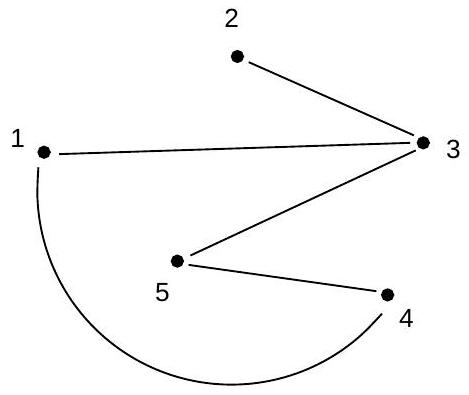
\includegraphics[max width=\textwidth, center]{2025_09_05_b69e29efaf9a6d2aa81ag-04}

Ejemplo 2: Consideremos el grafo dirigido $G=(V, E)$ donde $V=\{1,2,3,4,5,6\}$ y $E=\{(2,3),(3,2),(4,3),(3,5),(1,4),(4,5),(5,6),(6,1)\}$. En este caso los vértices 3 y 4 son adyacentes pero los vértices 2 y 4 no lo son.

Un grafo dirigido $G$ puede representarse gráficamente en el plano poniendo un punto por cada vértice de $G$ y una curva simple dirigida de $v$ y $w$ para cada rama $(v, w)$ de $G$. De esta manera, el grafo del ejemplo 2 puede representarse gráficamente en la forma\\
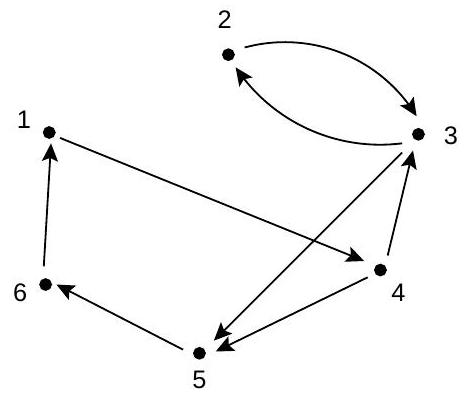
\includegraphics[max width=\textwidth, center]{2025_09_05_b69e29efaf9a6d2aa81ag-04(1)}

Definición: Dados un grafo $G=(V, E)$ y dados $v_{1}, v_{n} \in V$ diremos que una sucesión\\
$\mathcal{C}=\left(e_{1}, \ldots, e_{n-1}\right)$ de elementos de $E$ es un camino de $v_{1}$ a $v_{n}$ si $e_{i-1} \neq e_{i}$ para todo $2 \leq i \leq n-1$ y existen $v_{2}, \ldots v_{n-1} \in V$ tales que $e_{i}=\left(v_{i}, v_{i+1}\right)$ para todo $1 \leq i \leq n-1$. En tal caso diremos que $v_{1}, \ldots, v_{n}$ son los vértices del camino $\mathcal{C}$. Si $v_{i} \neq v_{j}$ para todo $i \neq j$ diremos que el camino es simple. Si $n \geq 3, v_{1}=v_{n}$ y $v_{1}, \ldots, v_{n-1}$ son todos distintos diremos que el camino es un ciclo o también que es un circuito.\\
En el grafo del ejemplo 1 , la sucesión $(2,3),(3,5),(5,4),(4,1)$ es un camino simple de 2 a 1 y la sucesión $(1,3),(3,5),(5,4),(4,1)$ es un ciclo. En el grafo del ejemplo 2 , la sucesión $(5,6),(6,1),(1,4),(4,3),(3,2),(2,3)$ es un camino de 5 a 3 . Este camino no es simple. La sucesión $(5,6),(6,1),(1,4),(4,5)$ es un ciclo. También lo es la sucesión $(2,3),(3,2)$.

Definición: Sea $G=(V, E)$ un grafo y sea $u \in V$. Definimos

$$
\begin{array}{ll}
i(u)=|\{v \in V /(v, u) \in E\}| & \text { indegree de } u \\
o(u)=|\{v \in V /(u, v) \in E\}| & \text { outdegree de } u
\end{array}
$$

y definimos el grado de $u$ como

$$
\delta(u)= \begin{cases}i(u)+o(u) & \text { si } G \text { es dirigido } \\ i(u) & \text { si } G \text { es no dirigido }\end{cases}
$$

Tanto en el caso dirigido como no dirigido resulta que $\delta(u)$ es la cantidad de ramas que inciden en $u$. (Observemos que si $G$ es no dirigido entonces los conjuntos que definen $i(u)$ y $o(u)$ son iguales y por eso no los contamos dos veces).\\
En el grafo del ejemplo 1 los vértices 1 , 4 y 5 tienen grado 2 , el vértice 2 tiene grado 1 y el vértice 3 tiene grado 3.\\
En el grafo del ejemplo 2 los vértices 1,2 y 6 tienen indegree 1 , outdegree 1 y grado 2 , el vértice 3 tiene indegree 2 , outdegree 2 y grado 4 , el vértice 4 tiene indegree 1 , outdegree 2 y grado 3 y el vértice 5 tiene indegree 2 , outdegree 1 y grado 3 .

Teorema: Sea $G=(V, E)$ un grafo no dirigido con $|V| \geq 2$. Entonces existen (al menos) dos vértices de $G$ que tienen el mismo grado.\\
Demostración: Sea $m=|V| \geq 2$. Entonces, para cada $v \in V$ se tiene que $\delta(v)$ puede ser $0,1,2, \ldots$ o $m-1$.

Primer caso: si $\delta(v) \geq 1$ para todo $v \in V$.\\
En este caso definimos una función $f: V \longrightarrow\{1,2, \ldots, m-1\}$ de un conjunto de $m$ elementos en un conjunto con $m-1$ elementos en la forma $f(v)=\delta(v)$. Luego, existen $v, w \in V, v \neq w$, tales que $\delta(v)=\delta(w)$.\\
Segundo caso: si $\delta(u)=0$ para algún $u \in V$.\\
En este caso $\delta(v)<m-1$ para todo $v \in V$ pues si $v \neq u$ entonces el conjunto de vértices que son adyacentes a $v$ no puede contener a $u$. Ahora también definimos una función\\
$f: V \longrightarrow\{0,1,2, \ldots, m-2\}$ de un conjunto de $m$ elementos en un conjunto con $m-1$ elementos en la forma $f(v)=\delta(v)$. Luego, $\exists v, w \in V, v \neq w$, tales que $\delta(v)=\delta(w)$.

Definición: Sea $G=(V, E)$ un grafo. Un subconjunto $S$ de $V$ se dice independiente si ningún par de elementos de $S$ son adyacentes.\\
En el grafo del ejemplo $1,\{1,2,5\}$ es un conjunto independiente. También lo es $\{2,4\}$. En el grafo del ejemplo $2,\{1,2,5\},\{2,4,6\}, \mathrm{y}\{3,6\}$ son conjuntos independientes.

Diremos que $S \subseteq V$ es un máximo conjunto independiente en $G$ si $S$ es independiente y $|S| \geq|T|$ para todo subconjunto independiente $T$ de $V$. Denotaremos por $\alpha(G)$ al cardinal de un máximo conjunto independiente en $G$.

Definición: Sea $G=(V, E)$ un grafo no dirigido. Definimos el número cromático de $G$, $\chi(G)$, como el mínimo número de colores que se necesitan para colorear los vértices de $G$ de forma tal que dos vértices adyacentes nunca tengan el mismo color.\\
Por ejemplo, si $K_{4}$ es el grafo completo no dirigido de 4 vértices\\
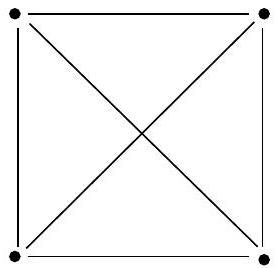
\includegraphics[max width=\textwidth, center]{2025_09_05_b69e29efaf9a6d2aa81ag-06(1)}\\
se tiene que $\chi\left(K_{4}\right)=4$, pero si consideramos el grafo $G$ que resulta de quitarle a $K_{4}$ una rama (y ningún vértice)\\
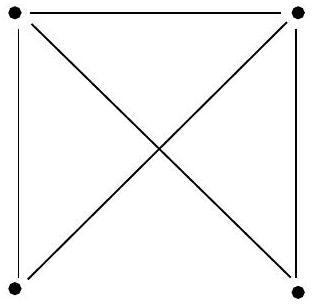
\includegraphics[max width=\textwidth, center]{2025_09_05_b69e29efaf9a6d2aa81ag-06}\\
entonces $\chi(G)=3$.\\
Teorema: Sea $G=(V, E)$ un grafo no dirigido con $m$ vértices. Entonces $\alpha(G) . \chi(G) \geq m$.\\
Demostración: Sea $n=\chi(G)$ y sea $f: V \longrightarrow\left\{a_{1}, \ldots, a_{n}\right\}$ una coloración de $G$ con $n$ colores. Entonces, por el principio de los casilleros, $\left|f^{-1}\left(a_{i}\right)\right| \geq \frac{|V|}{n}=\frac{m}{\chi(G)}$ para algún $i$ entre 1 y $n$. Pero $\alpha(G) \geq\left|f^{-1}\left(a_{j}\right)\right| \forall j=1,2, \ldots, n$ pues $S=f^{-1}\left(a_{j}\right)$ es un conjunto independiente (si $v, w \in f^{-1}\left(a_{j}\right)$ entonces $v$ y $w$ están pintados del mismo color y por lo tanto no pueden ser adyacentes). Luego, $\alpha(G) \geq \frac{m}{\chi_{(G)}}$ -\\
Nota: Un grafo no dirigido se dice planar si puede dibujarse en el plano de manera que sus ramas no se corten.\\
Por ejemplo, $K_{4}$ es un grafo planar pues puede dibujarse en el plano en la forma\\
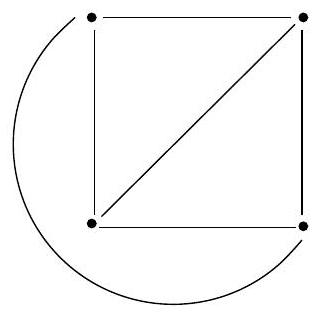
\includegraphics[max width=\textwidth, center]{2025_09_05_b69e29efaf9a6d2aa81ag-07}

Se sabe que si $G$ es un grafo planar entonces $\chi(G) \leq 4$. Luego, $\alpha(G) \geq \frac{|V|}{4}$.\\
A cada mapa le podemos asociar un grafo planar (no dirigido) $G=(V, E)$ donde $V$ es el conjunto de regiones del mapa y $E=\{(v, w) / v$ y $w$ tienen una frontera común $\}$.\\
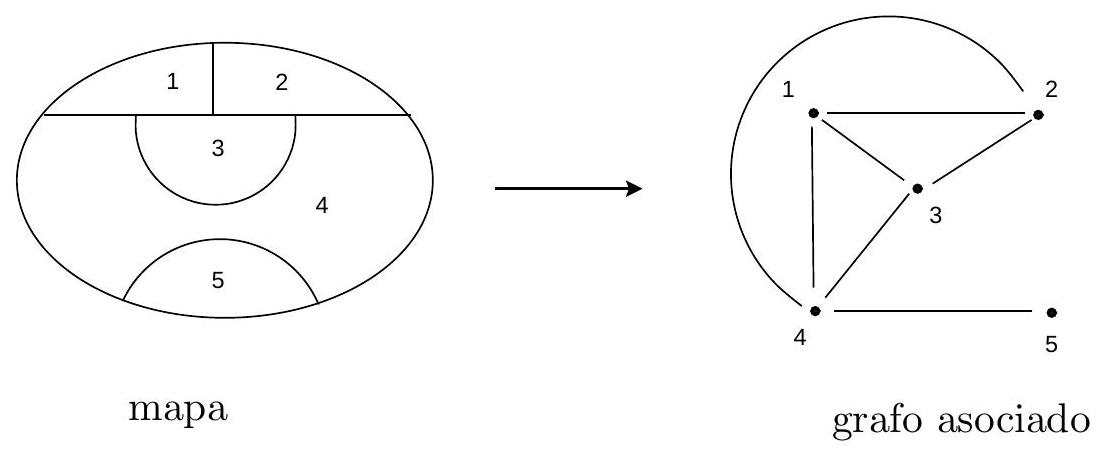
\includegraphics[max width=\textwidth, center]{2025_09_05_b69e29efaf9a6d2aa81ag-07(1)}

La desigualdad $\alpha(G) \geq \frac{|V|}{4}$ significa que un mapa con $m$ territorios necesariamente tiene al menos $\frac{m}{4}$ territorios que no tienen fronteras comunes dos a dos y $\chi(G) \leq 4$ significa que alcanzan 4 colores para colorear cualquier mapa de manera que dos regiones con una frontera común estén pintadas de distinto color.

Supongamos ahora que tenemos un grafo no dirigido con $2 n$ vértices que no contiene ningún triángulo (es decir, que no contiene ningún subconjunto de tres vértices que sean adyacentes dos a dos). ¿Cuál es el máximo número de ramas que puede tener $G$ ? Por ejemplo, consideremos el grafo bipartito no dirigido y completo $K_{n, n}$, cuyo conjunto de vértices es la unión disjunta de dos conjuntos de $n$ elementos $A$ y $B$ y donde ( $v, w$ ) es una rama si y sólo si $v \in A$ y $w \in B$. Por ejemplo, para $n=4$ el grafo bipartito no dirigido y completo $K_{4,4}$ es\\
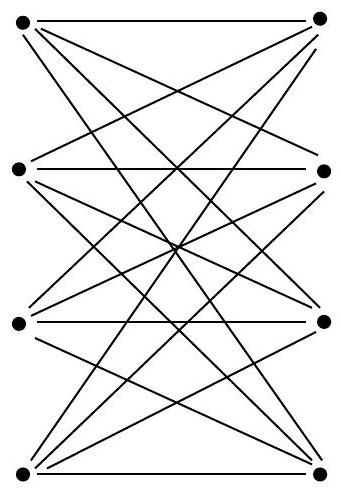
\includegraphics[max width=\textwidth, center]{2025_09_05_b69e29efaf9a6d2aa81ag-07(2)}

El grafo bipartito completo $K_{n, n}$ tiene $2 n$ vértices y no contiene ningún triángulo. Este grafo tiene $n^{2}$ ramas. Veremos que este es el máximo número de ramas posible.

Teorema: (Mantel, 1907) Si $G$ es un grafo no dirigido con $2 n$ vértices y al menos $n^{2}+1$ ramas entonces $G$ contiene un triángulo.

Demostración: Por inducción en $n$. Si $n=1$ entonces $G$ no puede tener $n^{2}+1$ ramas o más. Luego, la afirmación es cierta para $n=1$.\\
Supongamos ahora que vale para $n$ y sea $G$ un grafo con $2(n+1)$ vértices y $(n+1)^{2}+1$ ramas. Sean $u$ y $v$ dos vértices adyacentes de $G$ (siempre existen pues $G$ tiene al menos una rama, entonces los extremos de esa rama son adyacentes).\\
Sea $H$ el grafo que resulta de quitarle a $G$ los vértices $u$ y $v$ y todas las ramas que inciden en ellos. Si $H$ tiene al menos $n^{2}+1$ ramas entonces contiene un triángulo por hipótesis inductiva y por lo tanto $G$ contiene un triángulo. Supongamos entonces que $H$ tiene a lo sumo $n^{2}$ ramas y definamos la relación $\mathcal{R}$ de $A=\{u, v\}$ en $B=\{$ vértices de $H\}$ en la forma:

$$
(x, z) \in \mathcal{R} \text { si y sólo si } x \text { y } z \text { son adyacentes en } G
$$

Denotemos por $E(H)$ al conjunto de ramas de $H$ y por $E(G)$ al conjunto de ramas de $G$. Como $|\mathcal{R}|+1+|E(H)|=|E(G)|$ entonces

$$
|\mathcal{R}| \geq(n+1)^{2}+1-1-n^{2}=2 n+1
$$

Entonces, por el principio de los casilleros, existe $z \in B$ tal que

$$
\left|\mathcal{R}^{-1}(z)\right| \geq \frac{|\mathcal{R}|}{|B|} \geq \frac{2 n+1}{2 n}>1
$$

Luego, existe $z \in B$ tal que $\left|\mathcal{R}^{-1}(z)\right| \geq 2$. Esto significa que existe un vértice $z$ de $G$, $z \neq u, v$, tal que $(u, z) \in \mathcal{R}$ y $(v, z) \in \mathcal{R}$. Luego, $z$ es adyacente a $u$ y a $v$ en $G$ y, como $u$ y $v$ eran vértices adyacentes de $G$ entonces los vértices $z, u$ y $v$ forman un triángulo en $G$.

Veamos ahora una aplicación del principio de los casilleros que tiene que ver con coloraciones de los lattice points en el plano.

Teorema: Consideremos el conjunto de 21 lattice points en el plano $\{1,2, \ldots, 7\} \times\{1,2,3\}$ y supongamos que hemos coloreado cada uno de esos puntos de verde o de rojo. Entonces existen cuatro de esos puntos, todos del mismo color, que son los vértices de un rectángulo cuyos lados son paralelos a los ejes.

Demostración: Llamaremos columna a cualquier subconjunto de $\{1,2, \ldots, 7\} \times\{1,2,3\}$ formado por los tres puntos que tengan la misma primera coordenada. Diremos que un punto es el primer punto de una columna si es el que tiene segunda coordenada 1 , que es el segundo punto si es el que tiene segunda coordenada 2 y el tercer punto si es el que tiene segunda coordenada 3.\\
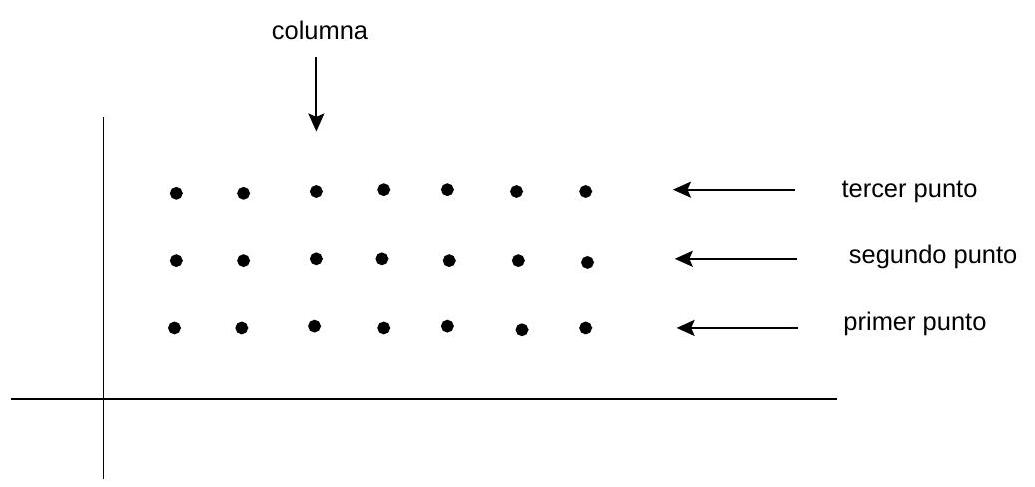
\includegraphics[max width=\textwidth, center]{2025_09_05_b69e29efaf9a6d2aa81ag-09}

Cada columna de 3 puntos contiene 3 puntos verdes o 2 verdes y 1 rojo o 1 verde y 2 rojos o 3 rojos. Luego, cada columna de 3 puntos contiene más puntos verdes que rojos o contiene más rojos que verdes. Llamemos V-columnas a las columnas que tienen más verdes que rojos y R -columnas a las otras.\\
Por el principio de los casilleros, hay al menos 4 V -columnas o al menos 4 R -columnas. En efecto, consideremos la función $f: A=\{$ columnas $\} \longrightarrow B=\{V, R\}$ definida por

$$
f(\mathcal{C})= \begin{cases}V & \text { si } \mathcal{C} \text { es una V-columna } \\ R & \text { si } \mathcal{C} \text { es una R-columna }\end{cases}
$$

Entonces se tiene que existe $b \in B$ tal que $\left|f^{-1}(b)\right| \geq \frac{|A|}{|B|}=\frac{7}{2}>3$. Luego, existe $b \in B$ tal que $\left|f^{-1}(b)\right| \geq 4$. Si $b=V$ esto dice que hay por lo menos 4 V -columnas y si $b=R$ que hay al menos 4 R -columnas. Sin pérdida de generalidad supongamos que hay por lo menos 4 V-columnas. Veremos que esto implica que hay 4 puntos verdes que son los vértices de un rectángulo de lados paralelos a los ejes.\\
Sea $g:\{\mathrm{V}$-columnas $\} \longrightarrow\{(V, V),(V, R),(R, V)\}$ la función definida por\\
$g(\mathcal{C})=($ color del primer punto de la columna $\mathcal{C}$, color del segundo punto de la columna $\mathcal{C})$\\
Entonces, por el principio de los casilleros, existe un elemento $b \in\{(V, V),(V, R),(R, V)\}$ tal que $\left|g^{-1}(b)\right| \geq \frac{4}{3}>1$, es decir, $\left|g^{-1}(b)\right| \geq 2$.\\
Si $b=(V, V)$ entonces existen al menos dos V -columnas con los primeros dos puntos verdes. Esos 4 puntos son todos verdes y son los vértices de un rectángulo de lados paralelos a los ejes.\\
Si $b=(V, R)$ entonces existen al menos dos V-columnas con el primer punto verde y el segundo rojo. Luego, el tercer punto de esas dos columnas debe ser verde. Tomando los primeros y terceros puntos de esas dos V-columnas se obtienen 4 puntos verdes que son los vértices de un rectángulo de lados paralelos a los ejes.\\
Finalmente, si $b=(R, V)$ entonces existen al menos dos V-columnas con el primer punto rojo y el segundo verde. Luego, el tercer punto de esas dos columnas debe ser verde. Tomando los segundos y terceros puntos de esas dos V-columnas se obtienen 4 puntos verdes que son los vértices de un rectángulo de lados paralelos a los ejes.

\section*{2. Sucesiones y órdenes parciales.}
Definición: Diremos que una sucesión finita de números reales $a_{1}, a_{2}, \ldots, a_{n}$ es monótona creciente (respectivamente decreciente) sii $a_{i} \leq a_{j}$ para todo $i<j$ (respectivamente, $a_{i} \geq a_{j}$ para todo $i<j$ ).

Teorema: (Erdös-Szekeres, 1935) Sean $m, n \in \mathbb{N}$. Entonces cualquier sucesión de números reales con $m . n+1$ términos $a_{1}, a_{2}, \ldots, a_{m . n+1}$ contiene una subsucesión monótona creciente de $m+1$ términos o contiene una subsucesión monótona decreciente de $n+1$ términos (o ambas).\\
Demostración: Supongamos que $a_{1}, a_{2}, \ldots, a_{m \cdot n+1}$ no contiene ninguna subsucesión monótona creciente de $m+1$ términos ni tampoco contiene ninguna subsucesión monótona decreciente de $n+1$ términos. Sea $f:\{1,2, \ldots, m . n+1\} \longrightarrow\{1,2, \ldots, m\} \times\{1,2, \ldots, n\}$ la función definida por $f(t)=\left(x_{t}, y_{t}\right)$, donde $x_{t}$ es la cantidad de términos que tiene la más larga de las subsucesiones monótonas crecientes de $a_{1}, a_{2}, \ldots, a_{m . n+1}$ que comienzan con $a_{t}$ y donde $y_{t}$ es la cantidad de términos que tiene la más larga de las subsucesiones monótonas decrecientes de $a_{1}, a_{2}, \ldots, a_{m \cdot n+1}$ que comienzan con $a_{t}$.\\
Por el principio de los casilleros, existen $j, k \in\{1,2, \ldots, m . n+1\}, j<k$, tales que $f(j)=f(k)$. Luego, $x_{j}=x_{k}$ e $y_{j}=y_{k}$. Veamos que esto no puede ocurrir.

Primer caso: $a_{j} \leq a_{k}$\\
En este caso, la subsucesión cuyo primer término es $a_{j}$ y los restantes términos son los de la subsucesión monótona creciente más larga que comienza con $a_{k}$ es una subsucesión monótona creciente de $1+x_{k}$ términos que comienza con $a_{j}$. Luego, $x_{j} \geq 1+x_{k}>x_{k}$.

Segundo caso: $a_{j} \geq a_{k}$\\
En este caso, la subsucesión cuyo primer término es $a_{j}$ y los restantes términos son los de la subsucesión monótona decreciente más larga que comienza con $a_{k}$ es una subsucesión monótona decreciente de $1+y_{k}$ términos que comienza con $a_{j}$. Luego, $y_{j} \geq 1+y_{k}>y_{k}$. ㅁ

Observación: Existe una sucesión de m.n términos que no contiene ninguna subsucesión monótona creciente de $m+1$ términos ni una subsucesión monótona decreciente de $n+1$ términos:\\
$n, n-1, \ldots, 2,1,2 n, 2 n-1, \ldots n+1,3 n, 3 n-1, \ldots, 2 n+1, \ldots, m . n, m . n-1, \ldots,(m-1) n+1$

Sea $X$ un conjunto y sea $\leq$ un orden parcial (es decir, una relación reflexiva, antisimétrica y transitiva) en $X$.\\
Definición: Un subconjunto $C$ de $X$ se llama una cadena (de $X$ ) si todo par de elementos de $C$ es comparable, es decir, si $\forall a, b \in C$ se verifica que $a \leq b$ o $b \leq a$. Si $C$ es una cadena con $|C|=k$, diremos que $C$ es una cadena de longitud $k$.

Definición: Un subconjunto $A$ de $X$ se llama una anticadena (de $X$ ) si ningún par de elementos de $A$ es comparable, es decir, si $\forall a, b \in A, a \neq b$, se verifica que $a \not \leq b$ y $b \not \leq a$. Si $A$ es una anticadena con $|A|=k$, diremos que $A$ es una anticadena de tamaño $k$.\\
La longitud y el ancho de un orden parcial $\leq$ se definen en la forma:

$$
\begin{array}{lr}
\lambda(\leq)=\max \{|C| / C \text { es una cadena }\} & \text { longitud } \\
\omega(\leq)=\max \{|A| / A \text { es una anticadena }\} & \text { ancho }
\end{array}
$$

Ejemplo: Sea $X=\{1,2,3, \ldots, 8\}$ y sea $\leq$ el orden parcial en $X$

$$
\{(3,1),(4,1),(4,3),(3,2),(4,2),(4,5),(6,5),(7,5),(7,6),(1,1),(2,2), \ldots,(8,8)\}
$$

Entonces $\{2,3\}$ y $\{5,6,7\}$ son cadenas y $\{7,1,8\}$ y $\{1,2,5,8\}$ son anticadenas. En este caso $\lambda(\leq)=3$ y $\omega(\leq)=4$.

Lema de Dilworth: Sea $\leq$ un orden parcial en un conjunto finito $X$ de al menos $m . n+1$ elementos. Entonces existe en $X$ una cadena de longitud $m+1$ o existe una anticadena de tamaño $n+1$.

Demostración: Supongamos que no existe en $X$ ninguna cadena de longitud $m+1$. Entonces podemos definir una función $f: X \longrightarrow\{1,2, \ldots, m\}$ en la forma:

$$
f(x)=\max \{|C| / C \text { es una cadena, } x \in C \text { y } z \leq x \forall z \in C\}
$$

Por el principio de los casilleros, existe $j \in\{1,2, \ldots, m\}$ tal que $\left|f^{-1}(j)\right| \geq \frac{m . n+1}{m}>n$, por lo tanto $\left|f^{-1}(j)\right| \geq n+1$. Veamos ahora que $A=f^{-1}(j)$ es una anticadena, lo que demuestra el lema ya que entonces cualquier subconjunto de $n+1$ elementos de $A$ será una anticadena de tamaño $n+1$.

Sean $a, b \in f^{-1}(j), a \neq b$. Luego, $f(a)=j=f(b)$. Queremos ver que $a \not \leq b$ y $b \not \leq a$. Supongamos que $a \leq b$. Sea $C$ una cadena tal que $a \in C, z \leq a \forall z \in C$ y $|C|=f(a)=j$. Entonces, $C \cup\{b\}$ es una cadena ya que si $y$ y $z$ son dos elementos de $C \cup\{b\}$ y ninguno de ellos es igual a $b$ entonces son comparables por ser $C$ una cadena, y si $y \in C$ y $z=b$ entonces son comparables pues $y \leq a$ y $a \leq b$, de donde $y \leq b=z$.\\
Además, como $a \leq b$ y $a \neq b$ entonces $b \notin C$ pues $z \leq a \forall z \in C$. Luego,

$$
|C \cup\{b\}|=|C|+1=f(a)+1=j+1=f(b)+1
$$

Pero entonces $C \cup\{b\}$ es una cadena, $b \in C \cup\{b\}$ y $z \leq b \forall z \in C \cup\{b\}$ (pues para todo $z \in C$ vale $z \leq a$ y estamos suponiendo $a \leq b$, de donde $z \leq b$ ). Luego, $f(b) \geq|C \cup\{b\}|=f(b)+1$, lo que es un absurdo. Hemos probado entonces que $a \not \leq b$. Análogamente se tiene que $b \not \leq a$.

Observación: La similitud entre el teorema de Erdös-Szekeres y el lema de Dilworth no es coincidencia. En realidad, puede probarse que el teorema resulta como corolario del lema (ver práctica 2).

El siguiente teorema es equivalente al lema de Dilworth.\\
Teorema: Sea $X$ un conjunto de $n$ elementos y sea $\leq$ un orden parcial en $X$ de longitud $\lambda y$ ancho $\omega$. Entonces $n \leq \lambda . \omega$

Demostración: Si fuese $n \geq \lambda \cdot \omega+1$ entonces, por el lema de Dilworth, existiría en $X$ una cadena de longitud $\lambda+1$ o una anticadena de tamaño $\omega+1$, lo que es una contradicción.

Observación: Hemos probado que el teorema se deduce del lema de Dilworth, pero en realidad son equivalentes (ver práctica 2 ).

Teorema de Dilworth: Sea $X$ un conjunto finito y sea $\leq$ un orden parcial en $X$ de longitud $\lambda$ y ancho $\omega$. Entonces $X$ es la unión disjunta de $\lambda$ anticadenas y también $X$ es la unión disjunta de $\omega$ cadenas.

Dejamos como ejercicio la demostración de que $X$ es la unión disjunta de $\lambda$ anticadenas. La demostración de que $X$ es la unión disjunta de $\omega$ cadenas puede consultarse en [Bo].\\
Corolario: Sea $\leq$ un orden parcial en un conjunto finito $X$ y sea $m$ el mínimo número de cadenas disjuntas que cubren $X$. Entonces $m=\omega(\leq)$.

Demostración: Sean $C_{1}, C_{2} \ldots, C_{m}$ cadenas disjuntas tales que $X=C_{1} \cup C_{2} \cup \ldots \cup C_{m}$. Sea $\omega=\omega(\leq)$ y sea $A=\left\{x_{1}, \ldots, x_{\omega}\right\}$ una anticadena de tamaño $\omega$. Luego, si $x_{i} \neq x_{j}$ entonces $x_{i}$ y $x_{j}$ no son comparables.\\
Consideremos la función $f: A \longrightarrow\{1,2, \ldots, m\}$ definida por

$$
f\left(x_{i}\right)=k \text { si y sólo si } x_{i} \in C_{k}
$$

Entonces $f$ está bien definida pues $C_{1}, C_{2}, \ldots, C_{m}$ son disjuntos y además es inyectiva. En efecto, si $f\left(x_{i}\right)=k=f\left(x_{j}\right)$, entonces $x_{i}, x_{j} \in C_{k}$. Luego $x_{i}$ y $x_{j}$ son comparables pues $C_{k}$ es una cadena, de donde debe ser $x_{i}=x_{j}$. Esto muestra que $\omega \leq m$.\\
Pero también vale que $m \leq \omega$ ya que, por el teorema de Dilworth, $X$ es la unión disjunta de $\omega$ cadenas.

Ejemplo: Sea $X=\{1,2,3, \ldots, 7\}$ y sea $\leq$ el orden parcial en $X$

$$
\{(3,1),(4,1),(4,3),(3,2),(4,2),(4,5),(6,5),(7,5),(7,6),(1,1),(2,2), \ldots,(7,7)\}
$$

y sea $G=(V, E)$ el grafo dirigido donde $V=X$ y $E=\{(x, y) \in V \times V / x \neq y$ y $x \leq y\}$, es decir, el grafo\\[0pt]
[Bo] Bollobás, B., Graph Theory, Cambridge Univ. Press, N.Y.\\
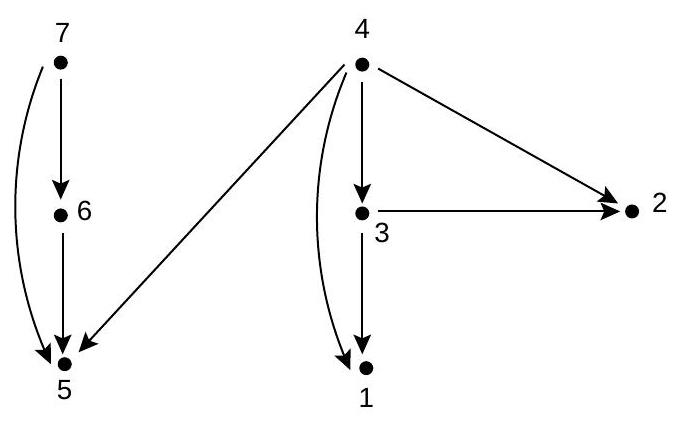
\includegraphics[max width=\textwidth, center]{2025_09_05_b69e29efaf9a6d2aa81ag-13}

Recordemos que un subconjunto $S$ de $V$ se dice independiente si ningún par de elementos de $S$ son adyacentes y que $\alpha(G)$ denota el cardinal de un máximo conjunto independiente en $G$.\\
En primer lugar, notemos que como $E=\{(x, y) \in V \times V / x \neq y$ y $x \leq y\}$ entonces un subconjunto $S$ de $V=X$ es independiente si y sólo si ningún par de elementos de $S$ son comparables, ya que dados dos elementos distintos $x$ e $y$, son adyacentes si y sólo si $x \leq y$ o $y \leq x$. Luego, $S$ es un subconjunto independiente de $V$ si y sólo si es una anticadena de $X$. Esto muestra que $\alpha(G)=\omega(\leq)$.\\
Además, un subconjunto $C$ de $X$ es una cadena si y sólo si los elementos de $C$ son los vértices de un camino en $G$. En efecto, si $C$ es una cadena entonces todo par de elementos de $C$ es comparable y, por lo tanto, podemos ordenar los elementos de $C$ de menor a mayor. Luego, $C=\left\{y_{1}, y_{2}, \ldots, y_{k}\right\}$ donde $y_{i} \leq y_{i+1}$. Luego, $y_{1} \longrightarrow y_{2} \longrightarrow \cdots \longrightarrow y_{k}$ es un camino en $G$ pues $\left(y_{i}, y_{i+1}\right) \in E(1 \leq i \leq k-1)$ y $C$ es el conjunto de vértices de ese camino.\\
Recíprocamente, si $y_{1} \longrightarrow y_{2} \longrightarrow \cdots \longrightarrow y_{k}$ es un camino en $G$ entonces $\left(y_{i}, y_{i+1}\right) \in E$ de donde $y_{i} \leq y_{i+1}(1 \leq i \leq k-1)$. Luego, por la transitividad, $y_{i} \leq y_{j}$ para todo $i<j$, de donde resulta que el conjunto de vértices de ese camino es una cadena en $X$.\\
Diremos que un conjunto de caminos en $G$ es disjunto por vértices si dos caminos de este conjunto nunca tienen un vértice en común. Diremos que un conjunto de caminos de $G$ cubren $V$ si todo $v \in V$ es un vértice de alguno de esos caminos.\\
Luego, si $\leq$ es un orden parcial en un conjunto $X$ y $G=(V, E)$ es el grafo donde $V=X$ y $E=\{(x, y) \in V \times V / x \neq y$ y $x \leq y\}$, entonces el mínimo número de caminos disjuntos por vértices de $G$ que cubren $V$ es igual al mínimo número de cadenas disjuntas que cubren $X$. Además, vimos que también vale $\omega(\leq)=\alpha(G)$. Luego, el corolario dice que, para este grafo $G$, el mínimo número de caminos disjuntos por vértices que cubren a $V$ es igual al cardinal de un máximo conjunto independiente en $G$.

Consideremos ahora el conjunto $T=\{1,2,3, \ldots, n\}$ donde $n$ es un número natural dado, y sea $X$ el conjunto cuyos elementos son los subconjuntos de $T$, parcialmente ordenado por inclusión. Nos preguntamos cuál es la longitud $\lambda$ y el ancho $\omega$ de este orden parcial en $X$. Calculemos primero su longitud. El subconjunto

$$
\{\emptyset,\{1\},\{1,2\},\{1,2,3\}, \ldots,\{1,2, \ldots, n\}\}
$$

es una cadena en $X$ de longitud $n+1$. Esto muestra que $\lambda \geq n+1$. Veamos que vale la igualdad.\\
Supongamos que $C \subseteq X$ es una cadena de longitud $k$. Entonces como todo par de elementos de $C$ es comparable, podemos ordenar los elementos de $C$ de menor a mayor. Luego, $C=\left\{S_{1}, S_{2}, \ldots, S_{k}\right\}$ con $S_{i} \subseteq S_{i+1}, S_{i} \neq S_{i+1}$. Entonces $\left|S_{1}\right|<\left|S_{2}\right|<\ldots<\left|S_{k}\right|$, de donde $\left|S_{2}\right| \geq\left|S_{1}\right|+1,\left|S_{3}\right| \geq\left|S_{2}\right|+1, \ldots,\left|S_{k}\right| \geq\left|S_{k-1}\right|+1$.\\
Luego, $\left|S_{k}\right| \geq\left|S_{1}\right|+k-1 \geq k-1$ y como $\left|S_{k}\right| \leq n$ pues $S_{k} \subseteq T$, entonces $k-1 \leq n$, es decir, $k \leq n+1$ y por lo tanto $\lambda \leq n+1$.\\
Hemos probado entonces que $\lambda=n+1$. Veamos ahora que $\omega=\binom{n}{\left[\frac{n}{2}\right]}$.\\
Lema: Sea $X$ el conjunto de partes del conjunto $T=\{1,2, \ldots, n\}$, parcialmente ordenado por inclusión. Si $S \in X$ es un subconjunto de $T$ de cardinal $k$ entonces hay exactamente $k!(n-k)!$ cadenas de longitud $n+1$ en $X$ que contienen a $S$.\\
Demostración: Sea $C$ una cadena de longitud $n+1$. Ordenando sus elementos de menor a mayor, $C=\left\{S_{1}, S_{2}, \ldots, S_{n+1}\right\}$ donde $S_{i} \subseteq S_{i+1}, S_{i} \neq S_{i+1}$. Como $\left|S_{n+1}\right| \leq n$ pues $S_{n+1} \subseteq T$ entonces debe valer que $\left|S_{i}\right|=i-1$ para todo $i$. En efecto, como


\begin{equation*}
\left|S_{i+1}\right| \geq\left|S_{i}\right|+1 \quad(1 \leq i \leq n) \tag{1}
\end{equation*}


entonces $\left|S_{2}\right| \geq\left|S_{1}\right|+1,\left|S_{3}\right| \geq\left|S_{2}\right|+1, \ldots,\left|S_{n+1}\right| \geq\left|S_{n}\right|+1$, de donde $\left|S_{n+1}\right| \geq\left|S_{1}\right|+n$. Si fuese $\left|S_{1}\right|>0$ entonces se tendría que $\left|S_{n+1}\right| \geq\left|S_{1}\right|+n>n$ y si en (1) valiera $>$ para algún $i$ entonces se tendría que $\left|S_{n+1}\right|>\left|S_{1}\right|+n$ de donde $\left|S_{n+1}\right|>n$. Luego $\left|S_{1}\right|=0$ y $\left|S_{i+1}\right|=\left|S_{i}\right|+1 \quad(1 \leq i \leq n)$ de donde resulta que $\left|S_{i}\right|=i-1$ para todo $i$.\\
Si además $C$ contiene a $S$ entonces $S_{i}=S$ para algún $i$, pero como $\left|S_{i}\right|=i-1$ y $|S|=k$ entonces $S=S_{k+1}$. Luego, $S_{1}, \ldots, S_{k+1} \subseteq S$ y $S \subseteq S_{k+2}, \ldots, S_{n+1}$. Además, como $S_{i} \subseteq S_{i+1}$ y $\left|S_{i}\right|=i-1$ para todo $i$, entonces

$$
\begin{aligned}
& S_{1}=\emptyset, S_{2}=\left\{a_{1}\right\}, S_{3}=\left\{a_{1}, a_{2}\right\}, \ldots, S_{k+1}=\left\{a_{1}, \ldots, a_{k}\right\}, \\
& S_{k+2}=\left\{a_{1}, \ldots, a_{k+1}\right\}, \ldots, S_{n+1}=\left\{a_{1}, \ldots, a_{k}, a_{k+1} \ldots a_{n}\right\}
\end{aligned}
$$

y como $S=S_{k+1}$ y $T=S_{n+1}$ (pues $S_{n+1} \subseteq T$ y $\left|S_{n+1}\right|=n$ ) entonces, denotando por $S^{\prime}$ al complemento de $S$ respecto de $T$, se tiene que $\left\{a_{1}, \ldots, a_{k}\right\}=S$ y $\left\{a_{k+1} \ldots a_{n}\right\}=S^{\prime}$. Recíprocamente, si $\left\{a_{1}, \ldots, a_{k}\right\}=S$ y $\left\{a_{k+1} \ldots a_{n}\right\}=S^{\prime}$, tomando

$$
\begin{aligned}
& S_{1}=\emptyset, S_{2}=\left\{a_{1}\right\}, S_{3}=\left\{a_{1}, a_{2}\right\}, \ldots, S_{k+1}=\left\{a_{1}, \ldots, a_{k}\right\}, \\
& S_{k+2}=\left\{a_{1}, \ldots, a_{k+1}\right\}, \ldots, S_{n+1}=\left\{a_{1}, \ldots, a_{k}, a_{k+1} \ldots a_{n}\right\}
\end{aligned}
$$

se tiene que $\left\{S_{1}, \ldots, S_{n+1}\right\}$ es una cadena de longitud $n+1$ que contiene a $S$.\\
Luego, las cadenas de longitud $n+1$ que contienen a $S$ son de la forma $\left\{S_{1}, \ldots, S_{n+1}\right\}$ con

$$
\begin{aligned}
& S_{1}=\emptyset, S_{2}=\left\{a_{1}\right\}, S_{3}=\left\{a_{1}, a_{2}\right\}, \ldots, S_{k+1}=\left\{a_{1}, \ldots, a_{k}\right\}, \\
& S_{k+2}=\left\{a_{1}, \ldots, a_{k+1}\right\}, \ldots, S_{n+1}=\left\{a_{1}, \ldots, a_{k}, a_{k+1} \ldots a_{n}\right\}
\end{aligned}
$$

donde $\left\{a_{1}, \ldots, a_{k}\right\}=S$ y $\left\{a_{k+1} \ldots a_{n}\right\}=S^{\prime}$. Por lo tanto hay exactamente $k!(n-k)$ ! cadenas de longitud $n+1$ que contienen a $S$.

Teorema: (Sperner, 1928) Sea $X$ el conjunto de partes del conjunto $\{1,2, \ldots, n\}$, parcialmente ordenado por inclusión. Si $A$ es una anticadena de tamaño $m$ entonces $m \leq\binom{ n}{\left[\frac{n}{2}\right]}$. Más aún, $\omega(\subseteq)=\binom{n}{\left[\frac{n}{2}\right]}$.\\
Demostración: Sea $A=\left\{A_{1}, A_{2}, \ldots, A_{m}\right\}$ una anticadena de tamaño $m$ y sea $k_{i}=\left|A_{i}\right|$. Entonces, por el lema, hay exactamente $k_{i}!\left(n-k_{i}\right)$ ! cadenas de longitud $n+1$ que contienen a $A_{i}$. Notemos que si $i \neq j$ las cadenas que contienen a $A_{i}$ son distintas de las cadenas que contienen a $A_{j}$ pues, si $i \neq j$, una cadena que contiene a $A_{i}$ no puede contener a $A_{j}$ ya que $A_{i}$ y $A_{j}$ no son comparables.\\
Además, como vimos en la demostración del lema, toda cadena de longitud $n+1$ necesariamente contiene a $\emptyset$. Por lo tanto, hay exactamente $n!$ cadenas de longitud $n+1$ pues la cantidad de cadenas de longitud $n+1$ es igual a la cantidad de cadenas de longitud $n+1$ que contienen a $\emptyset$ que, por el lema, es $0!(n-0)!=n!$. Luego,

$$
\sum_{i=1}^{m} k_{i}!\left(n-k_{i}\right)!\leq n!
$$

de donde

$$
\sum_{i=1}^{m} \frac{1}{\binom{n}{k_{i}}} \leq 1
$$

Como $\binom{n}{k_{i}} \leq\binom{ n}{\left[\frac{n}{2}\right]}$ para $1 \leq i \leq n$ entonces

$$
\frac{m}{\binom{n}{\left[\frac{n}{2}\right]}}=\sum_{i=1}^{m} \frac{1}{\binom{n}{\left[\frac{n}{2}\right]}} \leq \sum_{i=1}^{m} \frac{1}{\binom{n}{k_{i}}} \leq 1
$$

lo que prueba que $m \leq\binom{ n}{\left[\frac{n}{2}\right]}$.\\
Además, como dos conjuntos distintos de igual cardinal no son comparables entonces los $\binom{n}{\left[\frac{n}{2}\right]}$ subconjuntos de $\{1,2, \ldots, n\}$ de cardinal $\left[\frac{n}{2}\right]$ forman una anticadena lo que prueba que $\omega(\subseteq)=\binom{n}{\left[\frac{n}{2}\right]}$.

Nota: Si bien Sperner probó este teorema en 1928, la demostración que dimos, que es más sencilla, se debe a D. Lubell.\\
Veamos ahora cómo son las anticadenas de $X$ que tienen tamaño $\binom{n}{\left[\frac{n}{2}\right]}$. Es claro que si $n$ es par entonces el conjunto de todos los subconjuntos de $T$ de cardinal $\frac{n}{2}$ es una anticadena de tamaño $\binom{n}{\frac{n}{2}}=\binom{n}{\left[\frac{n}{2}\right]}$ ya que dos conjuntos distintos del mismo cardinal nunca son comparables.

Análogamente, si $n$ es impar entonces tanto el conjunto de todos los subconjuntos de $T$ de cardinal $\frac{n-1}{2}$ como el conjunto de todos los subconjuntos de $T$ de cardinal $\frac{n+1}{2}$ son anticadenas de tamaño $\binom{n}{\left[\frac{n}{2}\right]}$ ya que $\binom{n}{\frac{n+1}{2}}=\binom{n}{\frac{n-1}{2}}=\binom{n}{\left[\frac{n}{2}\right]}$.\\
Observación: Como vimos en la demostración del teorema, si $A=\left\{A_{1}, \ldots, A_{m}\right\}$ es una anticadena de tamaño $m$ y $k_{i}=\left|A_{i}\right|$ entonces

$$
\frac{m}{\binom{n}{\left[\frac{n}{2}\right]}}=\sum_{i=1}^{m} \frac{1}{\binom{n}{\left[\frac{n}{2}\right]}} \leq \sum_{i=1}^{m} \frac{1}{\binom{n}{k_{i}}} \leq 1
$$

Luego, $m=\binom{n}{\left[\frac{n}{2}\right]}$ sii $\binom{n}{\left[\frac{n}{2}\right]}=\binom{n}{k_{i}}$ para todo $i$, pues para todo $i$ vale que $\binom{n}{\left[\frac{n}{2}\right]} \geq\binom{ n}{k_{i}}$. Más aún, si $m=\binom{n}{\left[\frac{n}{2}\right]}$ entonces $\sum_{i=1}^{m} k_{i}!\left(n-k_{i}\right)!=n!$ pues

$$
\sum_{i=1}^{m} \frac{k_{i}!\left(n-k_{i}\right)!}{n!}=\sum_{i=1}^{m} \frac{1}{\binom{n}{k_{i}}}=\sum_{i=1}^{m} \frac{1}{\binom{n}{\left[\frac{n}{2}\right]}}=\frac{m}{\binom{n}{\left[\frac{n}{2}\right]}}=1
$$

Por lo tanto, si $m=\binom{n}{\left[\frac{n}{2}\right]}$ entonces toda cadena de longitud $n+1$ contiene exactamente un elemento de $A$.\\
En efecto, sabemos que hay $n!$ cadenas de longitud $n+1$. Por otra parte, la cantidad de cadenas de longitud $n+1$ que contienen algún elemento de $A$ es $\sum_{i=1}^{m} k_{i}!\left(n-k_{i}\right)!=n!$. Luego, toda cadena de longitud $n+1$ debe contener al menos un elemento de $A$ y, como una cadena no puede contener más de un elemento de $A$ entonces toda cadena de longitud $n+1$ contiene exactamente un elemento de $A$ como habíamos afirmado.

Teorema: Sea $X$ el conjunto de partes de $T=\{1,2, \ldots, n\}$, ordenado parcialmente por inclusión, y sea $A$ una anticadena de $X$ de tamaño $\binom{n}{\left[\frac{n}{2}\right]}$. Entonces se verifican:\\
i) Si $n$ es par entonces $A$ es el conjunto de todos los subconjuntos de $T$ de cardinal $\frac{n}{2}$.\\
ii) Si $n$ es impar entonces o bien $A$ es el conjunto de todos los subconjuntos de $T$ de cardinal $\frac{n-1}{2}$ o bien $A$ es el conjunto de todos los subconjuntos de $T$ de cardinal $\frac{n+1}{2}$.\\
Demostración: (Lovász) i) Supongamos que $n$ es par. Entonces $\left[\frac{n}{2}\right]=\frac{n}{2}$ de donde, por la observación, resulta que $\binom{n}{\frac{n}{2}}=\binom{n}{\left|A_{i}\right|}$ para cada $A_{i} \in A$. Luego $\left|A_{i}\right|=\frac{n}{2}$ para cada $A_{i} \in A$ y, por lo tanto, cada elemento de $A$ es un subconjunto de $T$ de cardinal $\frac{n}{2}$. Pero como $T$ tiene exactamente $\binom{n}{\frac{n}{2}}$ subconjuntos de cardinal $\frac{n}{2}$ y $A$ tiene tamaño $\binom{n}{\frac{n}{2}}$ entonces $A$ es igual al conjunto de todos los subconjuntos de $T$ de cardinal $\frac{n}{2}$.\\
ii) Supongamos que $n$ es impar. Entonces $\left[\frac{n}{2}\right]=\frac{n-1}{2}$ de donde, por la observación, resulta que $\binom{n}{\frac{n-1}{2}}=\binom{n}{\left|A_{i}\right|}$ para cada $A_{i} \in A$. Luego, si $A_{i} \in A$, se tiene que $\left|A_{i}\right|=\frac{n-1}{2}$ o $\left|A_{i}\right|=\frac{n+1}{2}$ ya que $\binom{n}{\frac{n-1}{2}}=\binom{n}{\frac{n+1}{2}}$.\\
Sea $k$ tal que $n=2 k+1$. Entonces $k=\frac{n-1}{2}=\left[\frac{n}{2}\right]$ y $k+1=\frac{n+1}{2}$. Luego, para cada $A_{i} \in A$ se tiene que $\left|A_{i}\right|=k$ o $\left|A_{i}\right|=k+1$. Como, por la observación, toda cadena de longitud $n+1$ contiene exactamente un elemento de $A$ entonces vale:\\
Si $U$ y $V$ son dos subconjuntos de $T$ tales que $U \subseteq V,|U|=k$ y $|V|=k+1$ entonces $U \in A$ y $V \notin A$ o $U \notin A$ y $V \in A$.\\
En efecto, si $U=\left\{a_{1}, \ldots, a_{k}\right\}, V=\left\{a_{1}, \ldots, a_{k}, a_{k+1}\right\}$ y $T-V=\left\{a_{k+2}, \ldots, a_{n}\right\}$ entonces, por la observación, la cadena de longitud $n+1$

$$
\left\{\emptyset,\left\{a_{1}\right\},\left\{a_{1}, a_{2}\right\}, \ldots,\left\{a_{1}, \ldots, a_{k}\right\},\left\{a_{1}, \ldots, a_{k+1}\right\},\left\{a_{1}, \ldots, a_{k+2}\right\}, \ldots,\left\{a_{1}, \ldots, a_{n}\right\}\right\}
$$

debe contener exactamente un elemento de $A$ y, como los elementos de $A$ tienen cardinal $k$ o $k+1$, entonces ese elemento es $\left\{a_{1}, \ldots, a_{k}\right\}=U$ o es $\left\{a_{1}, \ldots, a_{k+1}\right\}=V$. Luego, $U \in A$ y $V \notin A$ o $U \notin A$ y $V \in A$.\\
Veamos ahora que si $A$ contiene algún elemento de cardinal $k$ entonces contiene todos los subconjuntos de $T$ de cardinal $k$.\\
Supongamos entonces que existe $U \in A$ tal que $|U|=k$ y sea $U^{\prime}$ un subconjunto cualquiera de $T$ de cardinal $k$. Entonces existe una sucesión de subconjuntos

$$
U_{1}, V_{1}, U_{2}, V_{2}, \ldots, U_{m-1}, V_{m-1}, U_{m}
$$

tales que $U_{1}=U, U_{m}=U^{\prime},\left|U_{j}\right|=k \forall j=1,2, \ldots, m,\left|V_{j}\right|=k+1 \forall j=1,2, \ldots, m-1 \mathrm{y} U_{i}, U_{i+1} \subseteq V_{i} \forall i=1,2, \ldots, m-1$.\\
En efecto, si $U=\left\{a_{1}, \ldots, a_{r}, a_{r+1}, \ldots, a_{k}\right\}$ y si $U^{\prime}=\left\{a_{1}, \ldots, a_{r}, b_{r+1}, \ldots, b_{k}\right\}$, donde $\left\{a_{1}, \ldots, a_{r}\right\}=U \cap U^{\prime}$, entonces basta tomar $m=k-r+1, U_{1}=U, V_{1}=U_{1} \cup\left\{b_{r+1}\right\}$, $U_{2}=V_{1}-\left\{a_{r+1}\right\}, V_{2}=U_{2} \cup\left\{b_{r+2}\right\}, U_{3}=V_{2}-\left\{a_{r+2}\right\}, \ldots, V_{m-1}=U_{m-1} \cup\left\{b_{k}\right\}$, $U_{m}=V_{m-1}-\left\{a_{k}\right\}=U^{\prime}$.\\
Como $U_{1} \subseteq V_{1},\left|U_{1}\right|=k$ y $\left|V_{1}\right|=k+1$ y $U_{1}=U \in A$ entonces $V_{1} \notin A$, como $U_{2} \subseteq V_{1}$, $\left|U_{2}\right|=k$ y $\left|V_{1}\right|=k+1$ y $V_{1} \notin A$ entonces $U_{2} \in A$, como $U_{2} \subseteq V_{2},\left|U_{2}\right|=k$ y $\left|V_{2}\right|=k+1$ y $U_{2} \in A$ entonces $V_{2} \notin A$...\\
Luego, $V_{i} \notin A$ para todo $i=1, \ldots m-1$ y $U_{i} \in A$ para todo $i=1,2, \ldots, m$. En particular, $U^{\prime}=U_{m} \in A$.\\
Por lo tanto, si $A$ contiene algún elemento de cardinal $k$ entonces contiene todos los subconjuntos de $T$ de cardinal $k$ y, por lo tanto, $A$ es el conjunto de todos los subconjuntos de $T$ de cardinal $k=\frac{n-1}{2}$ pues $A$ tiene $\binom{n}{\left[\frac{n}{2}\right]}=\binom{n}{k}$ elementos.\\
Finalmente, si $A$ no contiene ningún elemento de cardinal $k$ entonces todos los elementos de $A$ tienen cardinal $k+1 \mathrm{y}$, por lo tanto, $A$ es el conjunto de todos los subconjuntos de $T$ de cardinal $k+1=\frac{n+1}{2}$ ya que $A$ tiene $\binom{n}{\left[\frac{n}{2}\right]}=\binom{n \frac{n}{2}}{\frac{n-1}{2}}=\binom{n}{\frac{n+1}{2}}=\binom{n}{k+1}$ elementos.

\section*{Teoría de Ramsey.}
Consideremos el grafo completo no dirigido de 6 vértices, al que denotaremos por $K_{6}$, y supongamos que coloreamos sus ramas de rojo o de verde. Entonces, en el grafo coloreado hay un triángulo verde o un triángulo rojo.\\
En efecto, elijamos un vértice cualquiera $v$ de $K_{6}$. Por el principio de los casilleros, hay por lo menos 3 de las 5 ramas que inciden en $v$ que tienen el mismo color. Supongamos entonces que las ramas $(v, x),(v, y)$ y $(v, z)$ son rojas. Si alguna de las ramas $(x, y),(y, z)$ o ( $x, z$ ) es roja, entonces hay un triángulo rojo $y$, si todas son verdes entonces hay un triángulo verde.\\
Dejamos como ejercicio mostrar que no ocurre lo mismo si en lugar de $K_{6}$ consideramos el grafo completo no dirigido $K_{5}$ de 5 vértices, es decir, mostrar que existe una manera de colorear las ramas de $K_{5}$ de rojo o verde sin que en el grafo coloreado haya un triángulo monocromático (es decir, un triángulo cuyas ramas sean todas del mismo color). Si denotamos por $K_{r}$ al grafo completo no dirigido de $r$ vértices, esto muestra que el mínimo $r$ tal que toda coloración rojo-verde de las ramas de $K_{r}$ contiene un grafo completo verde de 3 vértices o un grafo completo rojo de 3 vértices es $r=6$.

Teorema: (Ramsey, 1930) Dados $n, m \geq 2$, existe un mínimo entero $R(n, m)$ tal que toda coloración rojo-verde de las ramas del grafo completo no dirigido de $R(n, m)$ vértices contiene un grafo completo verde de $n$ vértices o un grafo completo rojo de $m$ vértices. Más aún, $R(n, m) \leq R(n-1, m)+R(n, m-1)$ para todo $n, m \geq 3$.\\
Demostración: Por inducción en $n$ y $m$.\\
Probaremos primero que $R(n, 2)=n$ y $R(2, m)=m$.\\
Si coloreamos las ramas de $K_{n}$ de rojo o verde entonces o bien todas las ramas son verdes o bien al menos una rama es roja. En el primer caso hay un $K_{n}$ verde y en el segundo hay un $K_{2}$ rojo. Esto muestra que $R(n, 2) \leq n$. Veamos ahora que vale la igualdad: si $r<n$ la coloración rojo-verde de $K_{r}$ que consiste en pintar todas las ramas de verde no contiene ningún $K_{n}$ verde ni ningún $K_{2}$ rojo. Análogamente se ve que $R(2, m)=m$.\\
Supongamos ahora que existen $R(n-1, m)$ y $R(n, m-1)$ y veamos que entonces existe $R(n, m)$ y satisface $R(n, m) \leq R(n-1, m)+R(n, m-1)$.\\
Supongamos que tenemos una coloración rojo-verde de las ramas del grafo completo de $R(n-1, m)+R(n, m-1)$ vértices, al que denotaremos por $G$ y sea $v$ un vértice cualquiera. Entonces, de las $R(n-1, m)+R(n, m-1)-1$ ramas de $G$ que inciden en $v$ hay al menos $R(n-1, m)$ que son verdes o al menos $R(n, m-1)$ que son rojas.\\
Si hay al menos $R(n-1, m)$ ramas verdes de $G$ que inciden en $v$, elijamos $R(n-1, m)$ vértices en el conjunto

$$
\{w /(v, w) \text { está pintada de verde }\}
$$

y consideremos el subgrafo completo de $G$ que tiene esos $R(n-1, m)$ vértices, con la coloración inducida. Entonces, por hipótesis inductiva, este subgrafo contiene un $K_{n-1}$\\
verde o un $K_{m}$ rojo. Si contiene un $K_{m}$ rojo entonces claramente $G$ contiene un $K_{m}$ rojo y si contiene un $K_{n-1}$ verde, agregando a ese $K_{n-1}$ verde el vértice $v$ y todas las ramas de $v$ a cada uno de los vértices de ese $K_{n-1}$, que sabemos que son verdes, se obtiene un $K_{n}$ verde.\\
De manera análoga se ve que si en $v$ inciden al menos $R(n, m-1)$ ramas rojas entonces hay un $K_{n}$ verde o un $K_{m}$ rojo.\\
Luego, $R(n, m)$ existe y satisface $R(n, m) \leq R(n-1, m)+R(n, m-1)$. $\square$\\
Los números $R(n, m)$ se llaman los números de Ramsey. Sólo pocos de ellos han sido calculados. Vimos antes que el mínimo $r$ tal que toda coloración rojo-verde de las ramas de $K_{r}$ contiene un grafo completo verde de 3 vértices o un grafo completo rojo de 3 vértices es $r=6$, es decir, que $R(3,3)=6$. También sabemos que $R(n, 2)=n$ y $R(2, m)=m$. Además, observemos que $R(n, m)=R(m, n)$.

Calculemos ahora $R(3,4)$. Por el teorema, sabemos que

$$
R(3,4) \leq R(2,4)+R(3,3)=4+6=10
$$

Veremos que $R(3,4)=9$. Para ello probaremos que toda coloración rojo-verde de $K_{9}$ contiene un $K_{3}$ verde o un $K_{4}$ rojo y dejaremos como ejercicio verificar que esto no vale para $K_{8}$.\\
Supongamos que existe una coloración rojo-verde de $K_{9}$ que no contiene ningún $K_{3}$ verde ni ningún $K_{4}$ rojo. Entonces, en cada vértice inciden a lo sumo 3 ramas verdes. En efecto, si en algún vértice $u$ incidieran 4 ramas verdes, $\left(u, v_{1}\right),\left(u, v_{2}\right),\left(u, v_{3}\right),\left(u, v_{4}\right)$, entonces, como no hay ningún $K_{3}$ verde, ninguna de las ramas ( $v_{i}, v_{j}$ ) puede ser verde. Luego, todas serían rojas y por lo tanto habría un $K_{4}$ rojo (el subgrafo completo con vértices $v_{1}, \ldots, v_{4}$ ). Además, en cada vértice inciden a lo sumo 5 ramas rojas. En efecto, si en algún vértice $u$ incidieran 6 ramas rojas, $\left(u, v_{1}\right),\left(u, v_{2}\right), \ldots,\left(u, v_{6}\right)$ entonces, como $R(3,3)=6$, el subgrafo completo con vértices $v_{1}, \ldots, v_{6}$ contendría un triángulo monocromático, que debe ser necesariamente rojo pues estamos suponiendo que no hay ningún $K_{3}$ verde. Si $v_{i}, v_{j}$ y $v_{k}$ son los vértices de ese triángulo rojo entonces el subgrafo completo con vértices $u, v_{i}, v_{j}, v_{k}$ sería un $K_{4}$ rojo.\\
Por lo tanto, en cada vértice inciden exactamente 3 ramas verdes y 5 ramas rojas. Luego, si consideramos el subgrafo $G$ de $K_{9}$ formado por los 9 vértices y todas las ramas verdes, entonces se tiene que cada vértice de $G$ tiene grado 3 . Esto implica que la suma de los grados de los vértices de $G$ es $3.9=27$, lo que contradice el hecho de que en cualquier grafo la suma de los grados de los vértices es par (ver ej. 13 de la práctica 6).

Como vimos, $R(n, m) \leq R(n-1, m)+R(n, m-1)$, lo que nos da una cota superior para $R(n, m)$ cuando conocemos $R(n-1, m)$ y $R(n, m-1)$. Sin embargo, tal como dijéramos, hay pocos números de Ramsey que se conocen, por lo cual sería deseable tener una cota que sólo dependiera de $n$ y $m$. El siguiente teorema proporciona esta cota:

Teorema: Si $n, m \geq 2$ entonces $R(n, m) \leq\binom{ n+m-2}{n-1}$.\\
Demostración: Por inducción en $n$ y $m$. Si $n=2$ entonces

$$
R(n, m)=R(2, m)=m=\binom{m}{1}=\binom{n+m-2}{n-1}
$$

y si $m=2$ entonces

$$
R(n, m)=R(n, 2)=n=\binom{n}{1}=\binom{n+m-2}{n-1}
$$

Supongamos ahora que la cota vale para $R(n-1, m)$ y para $R(n, m-1)$. Entonces

$$
\begin{aligned}
R(n, m) & =R(n-1, m)+R(n, m-1) \leq\binom{ n-1+m-2}{n-2}+\binom{n+m-1-2}{n-1}= \\
& =\binom{n+m-3}{n-2}+\binom{n+m-3}{n-1}=\binom{n+m-2}{n-1}
\end{aligned}
$$

En el caso particular en que $n=m$ se tiene la siguiente cota superior para los números de Ramsey $R(n, n)$, llamados diagonales

$$
R(n, n) \leq\binom{ 2 n-2}{n-1}=\binom{2(n-1)}{n-1} \leq 4^{n-1}
$$

Para obtener una buena cota inferior de los números de Ramsey diagonales recurriremos a un método probabilístico. La idea es ver a las coloraciones rojo-verde como eventos en un espacio de probabilidades y demostrar que una coloración que no contiene un subgrafo completo monocromático de un determinado tamaño ocurre con probabilidad mayor que cero.\\
Teorema: (método probabilístico) Si $\binom{r}{n}<2^{\binom{n}{2}-1}$ entonces $R(n, n)>r$.\\
Demostración: Supongamos que coloreamos al azar las ramas de $K_{r}$ de rojo o verde (para cada rama lanzamos una moneda, si sale cara pintamos la rama de rojo y si sale ceca de verde).\\
Para cada subgrafo completo $J$ de $n$ vértices sea $\mathcal{A}_{J}$ el evento " $J$ es monocromático". Entonces

$$
P\left(\mathcal{A}_{J}\right)=P(J \text { es verde })+P(J \text { es rojo })=\left(\frac{1}{2}\right)^{\binom{n}{2}}+\left(\frac{1}{2}\right)^{\binom{n}{2}}=\left(\frac{1}{2}\right)^{\binom{n}{2}-1}=\frac{1}{2^{\binom{n}{2}-1}}
$$

pues $J$ tiene $\binom{n}{2}$ ramas. Luego,

$$
P\left(\bigcup_{J} \mathcal{A}_{J}\right) \leq \sum_{J} P\left(\mathcal{A}_{J}\right)=\binom{r}{n} \cdot \frac{1}{2^{\binom{n}{2}-1}}
$$

pues $K_{r}$ tiene $\binom{r}{n}$ subgrafos completos de $n$ vértices.\\
Por lo tanto, si $\binom{r}{n}<2^{\binom{n}{2}-1}$ entonces $\left.P\left(\bigcup \mathcal{A}_{J}\right)\right)<1$. Luego, el complemento de $\bigcup \mathcal{A}_{J}$ ocurre con probabilidad positiva. En consecuencia, existe una coloración rojo-verde de $K_{r}$ que no contiene ningún $K_{n}$ monocromático, lo que prueba que $R(n, n)>r$. $\square$

Veamos ahora una generalización del teorema de Ramsey para $k$ colores.\\
Teorema: Sea $k \geq 2$. Dados $n_{1}, \ldots, n_{k} \geq 2$ existe un mínimo entero $R\left(n_{1}, \ldots, n_{k}\right)$ tal que toda coloración con $k$ colores $s_{1}, \ldots, s_{k}$ de las ramas del grafo completo con $R\left(n_{1}, \ldots, n_{k}\right)$ vértices contiene, para algún $i$ entre 1 y $k$, un subgrafo completo con $n_{i}$ vértices que tiene todas sus ramas del color $s_{i}$.\\
Más aún, $R\left(n_{1}, \ldots, n_{k}\right)$ satisface $R\left(n_{1}, \ldots, n_{k}\right) \leq R\left(R\left(n_{1}, \ldots, n_{k-1}\right), n_{k}\right)$ para todo $k \geq 3$.\\
Demostración: Por inducción en $k$. El caso $k=2$ es el teorema de Ramsey.\\
Supongamos ahora que vale para $k-1$ y supongamos que coloreamos el grafo completo con $R\left(R\left(n_{1}, \ldots, n_{k-1}\right), n_{k}\right)$ vértices con los colores $s_{1}, \ldots, s_{k}$. Si ahora cambiamos el color de todas las ramas de colores $s_{2}, \ldots, s_{k-1}$ por $s_{1}$ se obtiene una coloración con 2 colores del grafo completo con $R\left(t, n_{k}\right)$ vértices donde $t=R\left(n_{1}, \ldots, n_{k-1}\right)$. Luego, hay un subgrafo completo con $n_{k}$ vértices que tiene todas sus ramas de color $s_{k}$ o hay un subgrafo completo $K_{t}$ con $t=R\left(n_{1}, \ldots, n_{k-1}\right)$ vértices que tiene todas sus ramas de color $s_{1}$. Si ocurre lo primero entonces el grafo completo con $R\left(t, n_{k}\right)=R\left(R\left(n_{1}, \ldots, n_{k-1}\right), n_{k}\right)$ vértices contine un subgrafo completo con $n_{k}$ vértices que tiene todas sus ramas de color $s_{k}$ y si ocurre lo segundo, volviendo a pintar las ramas de $K_{t}$ de su color original, se obtiene un grafo completo con $t=R\left(n_{1}, \ldots, n_{k-1}\right)$ vértices cuyas ramas están pintadas con los $k-1$ colores $s_{1}, \ldots, s_{k-1}$ y que por lo tanto debe contener, para algún $i$ entre 1 y $k-1$, un subgrafo completo de $n_{i}$ vértices con todas sus ramas de color $s_{i}$ por hipótesis inductiva.\\
Por lo tanto, $R\left(n_{1}, \ldots, n_{k}\right)$ existe y satisface $R\left(n_{1}, \ldots, n_{k}\right) \leq R\left(R\left(n_{1}, \ldots, n_{k-1}\right), n_{k}\right)$. ㅁ Llamaremos números de Ramsey para $k$ colores a los números $R\left(n_{1}, \ldots, n_{k}\right)$.

Veamos ahora qué pasa cuando en lugar de ramas de un grafo coloreamos número naturales.\\
Lema de Schur: Sea $k \geq 1$. Entonces existe un mínimo entero $n=S(k)$ tal que toda coloración de los elementos de $\{1,2, \ldots, n\}$ con $k$ colores contiene una solución monocromática de la ecuación $x+y=z$, es decir, $\exists x, y, z \in\{1,2, \ldots, n\}$ (no necesariamente distintos), todos del mismo color, que verifican $x+y=z$.\\
Demostración: Dejamos como ejercicio comprobar que el lema es cierto para $k=1$ y supongamos que $k \geq 2$. Sea $m=R(3,3, \ldots, 3)-1$, donde $R(3,3, \ldots, 3)$ es el número de Ramsey que garantiza un triángulo monocromático en cualquier coloración con $k$ colores del grafo completo con $R(3,3, \ldots, 3)$ vértices.\\
Dada una coloración con $k$ colores de los elementos de $\{1,2, \ldots, m\}$, consideremos el grafo completo con los $m+1=R(3,3, \ldots, 3)$ vértices $1,2, \ldots, m+1$, donde pintamos cada rama $(i, j)$ del color que tiene el número $|i-j|$ (notar que $|i-j| \in\{1,2, \ldots, m\}$ ). Entonces\\
este grafo contiene un triángulo monocromático. Si $a, b, c$ son sus vértices, con $a<b<c$, entonces tomando $x=b-a, y=c-b$ y $z=c-a$ se tiene que $x, y, z \in\{1,2, \ldots, m\}$, todos son del mismo color (pues $x$ es del mismo color que la rama $(b, a), y$ es del mismo color que la rama ( $c, b$ ) y $z$ es del mismo color que la rama ( $c, a)$ ) y se verifica que $x+y=z$. Luego $S(k)$ existe y además satisface $S(k) \leq m$.

Los enteros $S(k)$ se llaman los números de Schur. Dejamos como ejercicio mostrar que $S(1)=2, S(2)=5$ y $S(3)=14$. El único otro número de Schur que se conoce es $S(4)=45$. Aunque este lema es considerado una parte importante de la teoría de Ramsey, Schur lo demostró pensando que podría utilizarlo para probar el último teorema de Fermat. Si bien Schur no consiguió probar el teorema de Fermat, utilizando este lema demostró que, cualquiera sea $n$, si $p$ es un primo tal que $p>S(n)$ entonces la ecuación $x^{n}+y^{n}=z^{n}$ tiene una solución no trivial módulo $p$.

Definición: Una progresión aritmética de longitud $m$ es una sucesión de $m$ términos $a_{1}, \ldots, a_{m}$ tales que $a_{2}-a_{1}=a_{3}-a_{2}=a_{4}-a_{3}=\cdots=a_{m}-a_{m-1}$, es decir, una sucesión del tipo

$$
a, a+d, a+2 d, \ldots, a+(m-1) d
$$

Teorema: (Van der Waerden) Dados $k, m \in \mathbb{N}$ existe un mínimo entero $n=W(k, m)$ tal que para toda coloración de los elementos de $\{1,2, \ldots, n\}$ con $k$ colores el conjunto $\{1,2, \ldots, n\}$ contiene una progresión aritmética monocromática de longitud $m$.\\
No daremos la demostración ya que es bastante compleja. También vale la siguiente generalización del teorema de Van der Waerden:\\
Teorema: Sean $k, m \in \mathbb{N}$. Entonces toda coloración de los números naturales con $k$ colores contiene una progresión aritmética monocromática de longitud $m$.

Los enteros $W(k, m)$ se llaman los números de Van der Waerden. Lamentablemente no se conocen buenas cotas para ellos y los únicos que se han podido calcular son $W(1, m)=m$, $W(k, 1)=1, W(k, 2)=k+1, W(2,3)=9, W(3,3)=27, W(4,3)=76, W(2,4)=35$ y $W(2,5)=178$. Schur ya había conjeturado que cualquier coloración de los números números naturales contiene una progresión aritmética monocromática arbirtariamente larga antes de que Van der Waerden probara el teorema.


\end{document}